 %%
 % COMAP2024SCUT template
 % Created by Caibin Zeng, email: macbzeng@scut.edu.cn  %
 % January 8, 2025
 %%
 
 %美赛模板:正文部分

 \documentclass[12pt]{article}  % 官方要求字号不小于 12 号,此处选择 12 号字体
 % \linespread{1.1}
 % \bibliographystyle{plain}
 % 本模板不需要填写年份,以当前电脑时间自动生成
 %%%%%%%%%%%%%%%%%%%%%%%%%%%%%%%%%%%%%%%%%%%%%%%%%%%%%%%%%%%%%%%%%%%%%%%%%%%%%%%
 % 请在以下的方括号中填写队伍控制号
 \usepackage[2511654]{easymcm}  % 载入 EasyMCM 模板文件
 \problem{B}  % 请在此处填写题号
 %%%%%%%%%%%%%%%%%%%%%%%%%%%%%%%%%%%%%%%%%%%%%%%%%%%%%%%%%%%%%%%%%%%%%%%%%%%%%%%%
 % \usepackage{mathptmx}  % 这是 Times 字体,中规中矩 
 \usepackage{palatino}  % mathpazo 这palatino是 COMAP 官方杂志采用的更好看的 Palatino 字体,可替代以上的 mathptmx 宏包
 \usepackage{pdfpages}
 \usepackage{longtable}
 \usepackage{tabu}
 \usepackage{threeparttable}
 \usepackage{listings}
 \usepackage{paralist}
 \usepackage{hyperref}
 \usepackage[linesnumbered,ruled,vlined]{algorithm2e}
 \usepackage{subfigure}
 \usepackage{subcaption}
 \usepackage{cleveref} %可以调用
 \usepackage{tcolorbox}
 \tcbuselibrary{most}
 \newtcolorbox{mybox}[2][]{colbacktitle=red!10!white, colback=blue!10!white,coltitle=red!70!black, title={#2},fonttitle=\bfseries,#1}
 \graphicspath{{img/}}          % 此处{img/}为相对路径,注意加上“/”
  \let\itemize\compactitem
  \let\enditemize\endcompactitem
 \newcommand{\upcite}[1]{\textsuperscript{\textsuperscript{\cite{#1}}}}
 
 
 \title{The Title Should be Concise and Informative}  % 标题
 
 % 如需要修改题头(默认为 MCM/ICM),请使用以下命令(此处修改为 MCM)
 %\renewcommand{\contest}{MCM}
 
  %文档开始
 \begin{document}
 
 % 此处填写摘要内容
 \begin{abstract}
     
 
 
    Juneau City in Alaska, USA is facing the problem of overtourism. The number of tourists and tax rates need to be adjusted to improve the satisfaction of tourists and residents. The government has implemented some measures to limit the number of tourists, protect the environment, and improve local infrastructure, but the results have not been satisfactory due to the complex factors affecting tourist and resident satisfaction.
     
 First of all, the \textbf{title} of your manuscript is usually the first introduction readers (and reviewers) have to your work. Therefore, you must select a title that grabs attention, accurately describes the content of your manuscript, and makes people want to read further. An effective title should:
 \begin{itemize}
     \setlength{\parsep}{0ex} %段落间距
     \setlength{\topsep}{2ex} %列表到上下文的垂直距离
     \setlength{\itemsep}{1ex} %条目间距
     \item Convey the main topics of the study
     \item Highlight the importance of the research
     \item Be concise
     \item Attract readers
 \end{itemize}
 
 Secondly, the \textbf{summary} is a guide to the most important parts of your content and it has to be able to stand alone. As a time-saving shortcut for referees, it needs to contain enough information about the paper to allow referees to make a judgement. 
   
 A well-written and complete solution should contain the background, your contributions, model assumptions and reasons, useful notations and interpretations, data preprocessing if necessary, build and solve the reasonable models for each task or problem, sensitivity/error/robustness analysis, model evaluation including strengths and weaknesses, special requirement (Letter of Recommendations), references list and any appendices (optional). 
 
 For each task, please present the specific model and avoid using complicated or obscure one. Meanwhile, you shold answer these questions for each task:
 \begin{itemize}
     \setlength{\parsep}{0ex} %段落间距
     \setlength{\topsep}{2ex} %列表到上下文的垂直距离
     \setlength{\itemsep}{1ex} %条目间距
     \item What was done?
     \item Why did you choose the model?
     \item What did you find?
     \item Why are these findings useful and important?
 \end{itemize}
 
 Answering these questions lets referees know the most important points about your work, and helps them decide whether they want to read the rest of your solution. 
 
 Additionly, the \textbf{keywords} can help indexers and search engines find relevant papers. However, to be effective, keywords must be chosen carefully. They should:
 \begin{itemize}
     \setlength{\parsep}{0ex} %段落间距
     \setlength{\topsep}{2ex} %列表到上下文的垂直距离
     \setlength{\itemsep}{1ex} %条目间距
     \item Represent the content of your work
     \item Be specific and recognizable within related field 
 \end{itemize}
 
 Finally, make sure you keep it one-page summary sheet and a 25-page limit for your whole PDF solution.
 
     % 此处填写关键字,以分号分开
     \vspace{5pt}  %mm	毫米	1 mm = 2.845 pt   pt 点	1 pt = 0.351 mm
     \textbf{Keywords}: ARIMA; Markov chain; Drought resistance; Faciliation model; multiple objective programming model
 
 \end{abstract}
 
 \maketitle  % 生成 Summary Sheet
 
 \tableofcontents  % 生成目录
 
 
 % 正文开始
 % Chapter 1: Introduction
 \section{Introduction}
 
 This is the first part of your work, which can be divided into three subsections: background, restatement of the problem and our work. It should be emphasized that you do not copy the original information including words and pictures. You may delete these instructions as you begin to type your report here.
 
 \subsection{Background}
 
 In the \textbf{Background} subsection, you need to extract the essential information from the problem sheet and consult relevant literatures.  Precisely, you provide a paragraph composed of 3 or 4 sentences with 2-4 references \cite{NDZY2021,V2020}. If necessary, you could present an illustration by yourselves or from some reference.  
 
 
 \subsection{Restatement of the Problem}
 
 In the \textbf{Restatement of the Problem} subsection, you just need a transition sentence and itemize the restatements using the 
 verb-object structure. 
 
 This is an example for the transition sentence: \textit{Considering the background information and limiting conditions identified in the problem statements, we are supposed to address the following issues:}. 
 
 \subsection{Our Work}
 
 In the \textbf{Our Work} subsection, you should present a transition sentence, itemize your contributions and a flow chart describing your work. 
 
 This is an example for the transition sentence:  \textit{To avoid complicated description, intuitively reflect our work process, the flow chart is shown as Figure \ref{fig1}}.
  
 
 
 \begin{figure}[htbp]  %h此处,t页顶,b页底,p独立一页,浮动体出现的位置 [H]
 
 \centering  %图表居中
 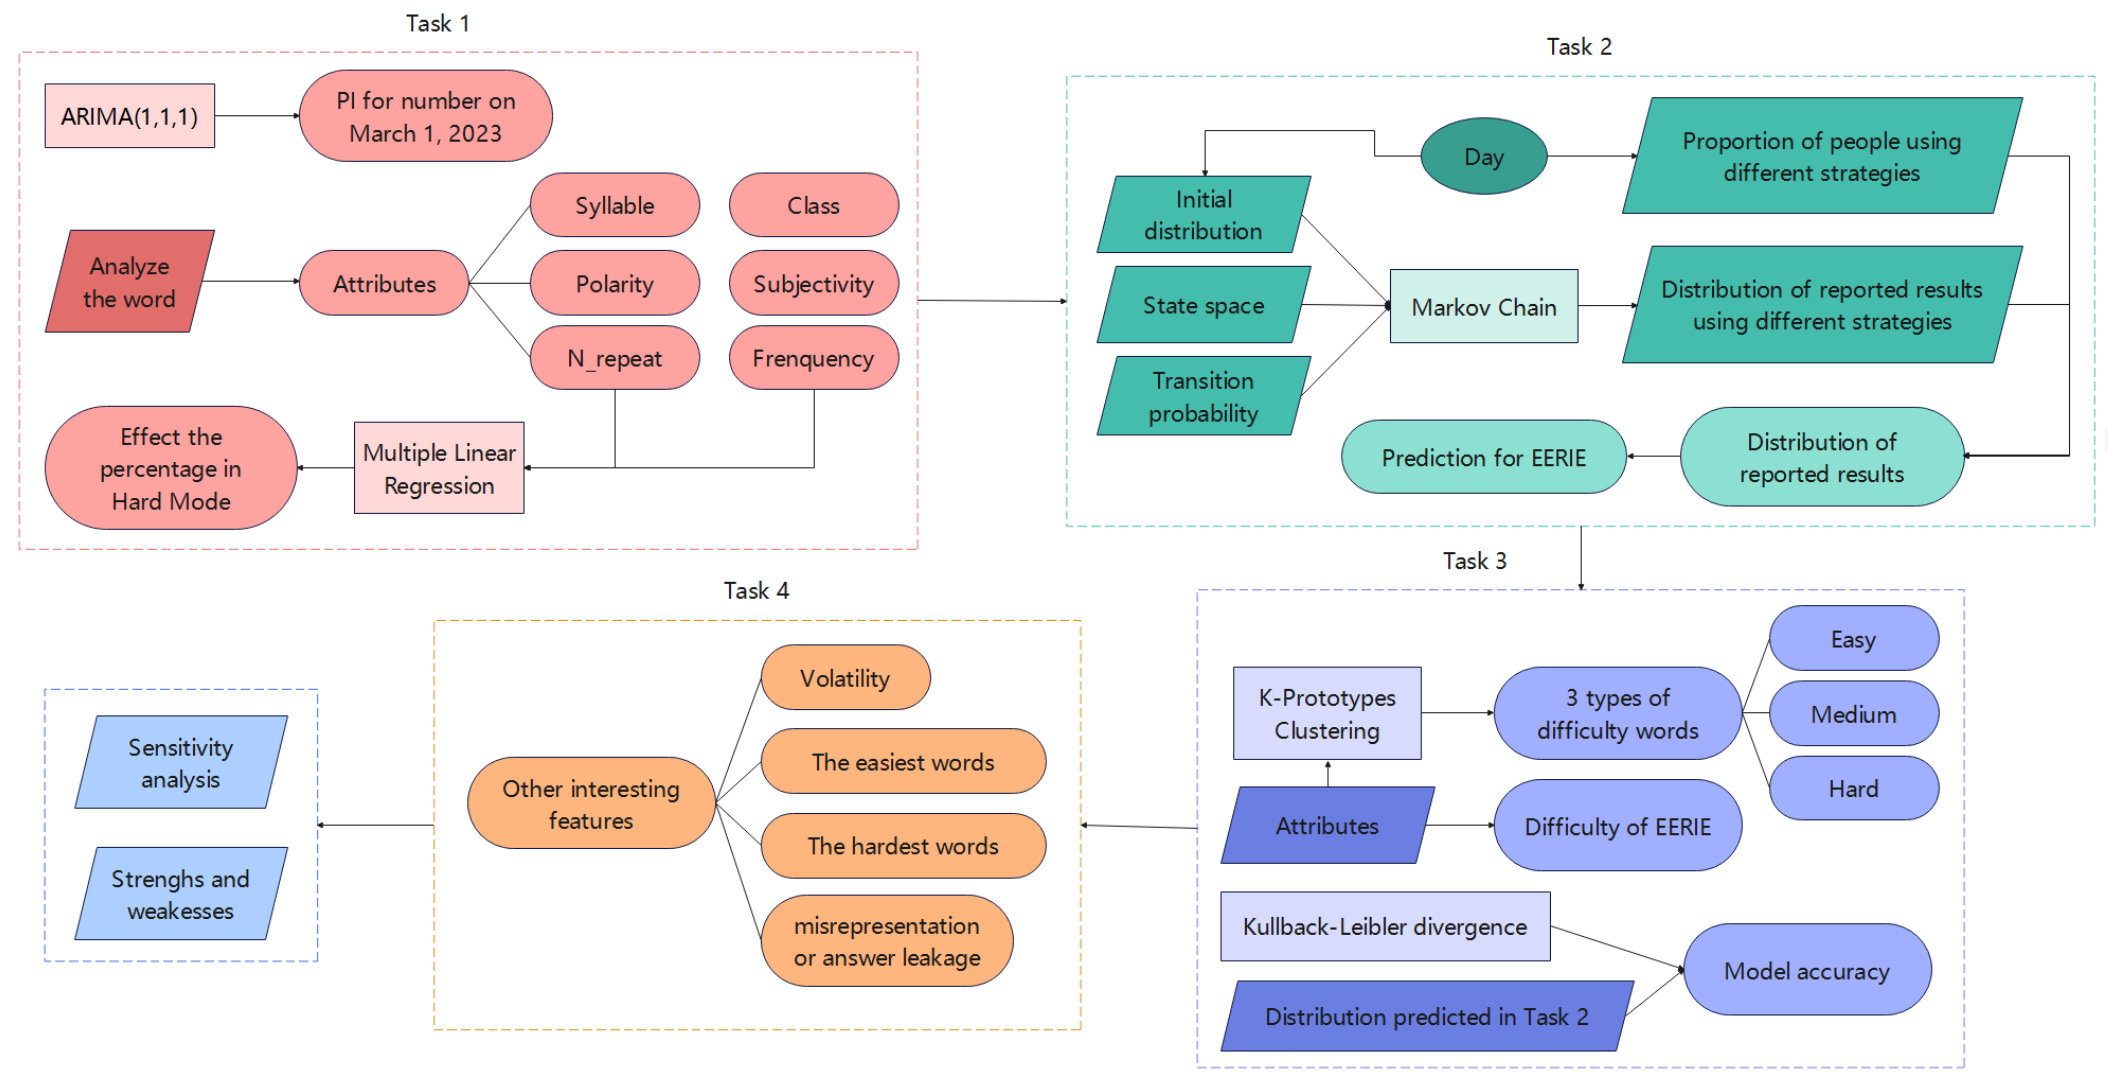
\includegraphics[width=.9\textwidth]{Flow_Chart.png} %图片的名称或者路径之中有空格会出问题 
 \caption{Flow Chart of Our Work (From Team \# 2318982)} % 图片标题 
 \label{fig1}%交互引用
 \end{figure}
 
 
 \section{Assumptions and Explanations}
 
 In this section, we need to make reasonable assumptions to simplify the problem and facilitate the modelling, and each hypothesis is closely followed by its appropriate explanation.
 
 \begin{itemize}
     \setlength{\parsep}{0ex} %段落间距
     \setlength{\topsep}{2ex} %列表到上下文的垂直距离
     \setlength{\itemsep}{1ex} %条目间距
     \item[\bfseries \textit{Assumption} 1:]  XXX
     \item[\bfseries \textit{Explanation:}]  XXX
     \vspace{1ex}
     \item[\bfseries \textit{Assumption} 2:]  XXX
     \item[\bfseries \textit{Explanation:}]  XXX
     \vspace{1ex}
         \item[\bfseries \textit{Assumption} 3:]  XXX
     \item[\bfseries \textit{Explanation:}]  XXX
 \end{itemize}
 
 Additional assumptions are made to simplify the analysis for individual sections. These assumptions will be discussed at the appropriate locations.
 
 \section{Notations}
 Some important mathematical notations used in this paper are listed in Table \ref{tab1}. 
 \begin{table}[htbp]
 \begin{center}
 \caption{Notations used in this paper}
 \begin{tabular}{cl} % 第一列居中对齐、第二列居左对齐
 \toprule[2pt]
 \multicolumn{1}{m{4cm}}{\centering Symbol}
 &\multicolumn{1}{m{10cm}}{\centering Description }\\  %3cm 和 8cm 是列宽,根据实际需求修改
 \midrule
 $x_i$   & XXXXX \\
 $y_i$   & YYYYYY \\
 \bottomrule[2pt]
 \end{tabular}	\label{tab1} % 交互引用 
  \begin{tablenotes}
         \footnotesize
         \item[*] *\href{https://www.caam.rice.edu/~heinken/latex/symbols.pdf}{ \LaTeX~Mathematical symbols collected by Prof. M. Heinkenschloss}. %此处加入注释*信息
       \end{tablenotes}
 \end{center}
 \end{table} 
 \vspace{-1cm} 
 
 
 
 \section{Data Preprocessing}
 
 This section is optional and the following texts are extracted from MonkeyLearn Blog \cite{Mesevage2021}. Data preprocessing is a step in the data mining and data analysis process that takes raw data and transforms it into a format that can be understood and analyzed by computers and machine learning.
 
 Raw, real-world data in the form of text, images, video, etc., is messy. Not only may it contain errors and inconsistencies, but it is often incomplete, and doesn’t have a regular, uniform design.
 
 So calculating structured data, like whole numbers and percentages is easy. However, unstructured data, in the form of text and images must first be cleaned and formatted before analysis.
 
 Depending on your data gathering techniques and sources, you may end up with data that’s out of range or includes an incorrect feature, like household income below zero or an image from a set of “zoo animals” that is actually a tree. Your set could have missing values or fields. Or text data, for example, will often have misspelled words and irrelevant symbols, URLs, etc.
 
 \begin{figure}[htbp]  %h此处,t页顶,b页底,p独立一页,浮动体出现的位置
     
     \centering  %图表居中
     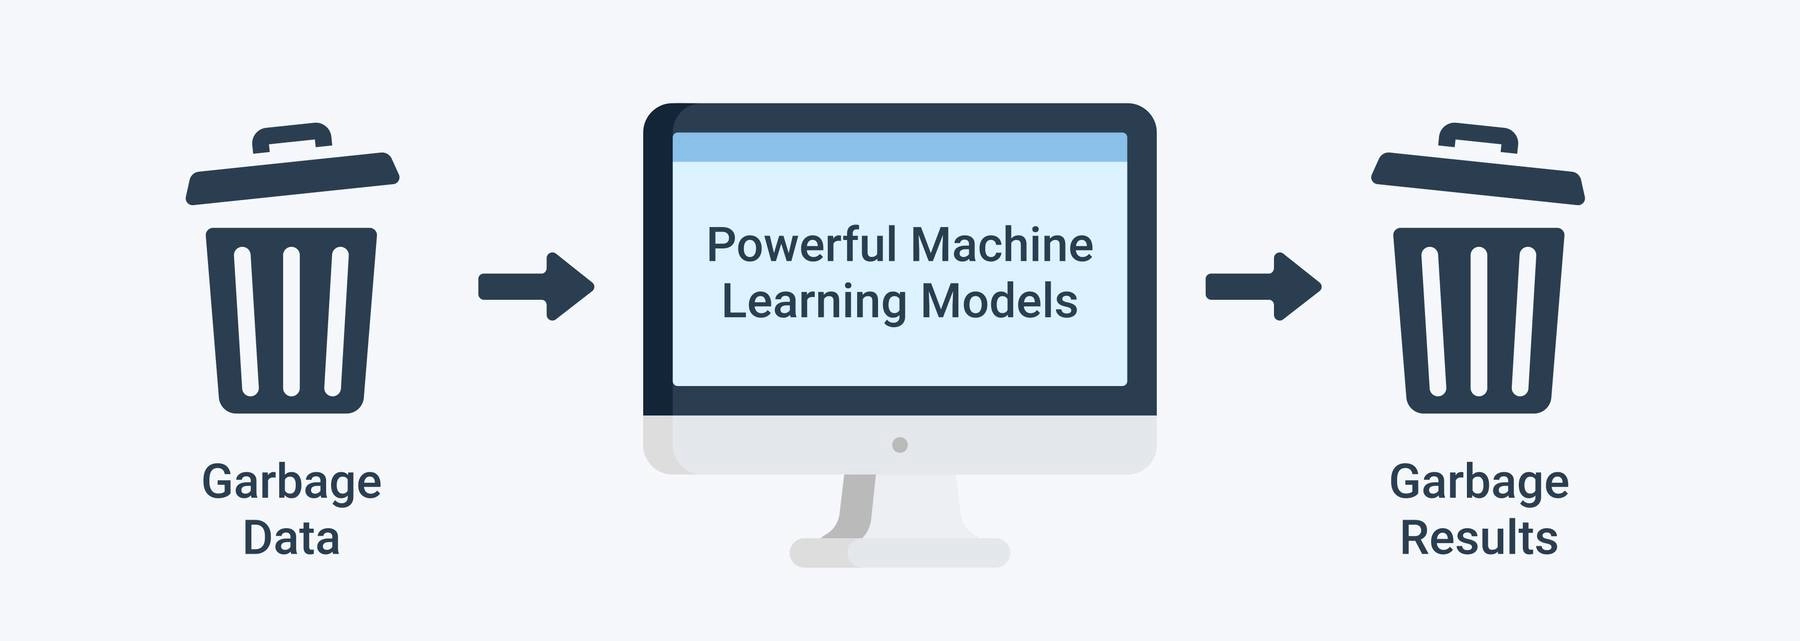
\includegraphics[width=.7\textwidth]{DataProc.jpg} %图片的名称或者路径之中有空格会出问题 
     \caption{Why data preprocessing is importance? (From MonkeyLearn Blog)} % 图片标题 
     \label{fig2}%交互引用
 \end{figure}
  
 
 Data sets can be explained with or communicated as the features that make them up. This can be by size, location, age, time, color, etc. Features appear as columns in datasets and are also known as attributes, variables, fields, and characteristics. 
 
 It’s important to understand what features are when preprocessing your data because you’ll need to choose which ones to focus on depending on what your business goals are. 
 
 There are the two different types of features that are used to describe data: categorical and numerical.
 
 \begin{itemize}
     \setlength{\parsep}{0ex} %段落间距
     \setlength{\topsep}{2ex} %列表到上下文的垂直距离
     \setlength{\itemsep}{1ex} %条目间距
 \item [\textbf{Categorical features:}] Features whose explanations or values are taken from a defined set of possible explanations or values. Categorical values can be colors of a house; types of animals; months of the year; True/False; positive, negative, neutral, etc. The set of possible categories that the features can fit into is predetermined.
 \item [\textbf{Numerical features: }]
 Features with values that are continuous on a scale, statistical, or integer-related. Numerical values are represented by whole numbers, fractions, or percentages. Numerical features can be house prices, word counts in a document, time it takes to travel somewhere, etc.
 
 Let’s take a look at the established steps you’ll need to go through to make sure your data is successfully preprocessed.
 
 \begin{enumerate}[(1)]
         \setlength{\parsep}{0ex} %段落间距
     \setlength{\topsep}{2ex} %列表到上下文的垂直距离
     \setlength{\itemsep}{1ex} %条目间距
     \item Data quality assessment: data anomalies and inherent problems
     \begin{itemize}
         \setlength{\parsep}{0ex} %段落间距
         \setlength{\topsep}{2ex} %列表到上下文的垂直距离
         \setlength{\itemsep}{1ex} %条目间距
         \item Mismatched data types
         \item Mixed data values
         \item Data outliers
         \item Missing data
     \end{itemize}
     \item Data cleaning: adding missing data and correcting, repairing, or removing incorrect or irrelevant data
     \begin{itemize}
     \setlength{\parsep}{0ex} %段落间距
     \setlength{\topsep}{2ex} %列表到上下文的垂直距离
     \setlength{\itemsep}{1ex} %条目间距
     \item Missing data: Ignore the tuples or Manually fill in 
     \item Noisy data: Binning or Regression or Clustering 
 \end{itemize}
     \item Data transformation: turning the data into the proper format(s) needed
     \begin{itemize}
         \setlength{\parsep}{0ex} %段落间距
         \setlength{\topsep}{2ex} %列表到上下文的垂直距离
         \setlength{\itemsep}{1ex} %条目间距
         \item Aggregation: combines together in a uniform format
         \item Normalization: scales your data into a regularized range
         \item Feature selection: chooses the important features
         \item Discreditization: pools data into smaller intervals
         \item Concept hierarchy generation: add a new hierarchy
     \end{itemize}
     \item Data reduction
 \begin{itemize}
     \setlength{\parsep}{0ex} %段落间距
     \setlength{\topsep}{2ex} %列表到上下文的垂直距离
     \setlength{\itemsep}{1ex} %条目间距
     \item Attribute selection: combines tags or features
     \item Numerosity reduction: helps with data storage and transmission
     \item Dimensionality reduction: reduces the amount of data 
 \end{itemize}
 \end{enumerate}
 
 
 
 
 
 
 \end{itemize}
 
 \section{Modelling, solving, evaluating and predicting}
 
 You need to several sections to model, solve, evaluate and predict each task or problem. In the following, we shall review some helpful information to this respect.
 
 \subsection{Introduction to MCM/ICM}
 
 COMAP's Mathematical Contest in Modeling (MCM)/ Interdisciplinary Contest in Modeling (ICM) is an international contest designed to provide undergraduate students with the opportunity to work as team members to engage in and improve their modeling, problem solving, and writing skills. Teams apply mathematics to model, develop, and communicate a solution to a real-world problem.
 
 Contest teams of up to three students address one of the following six problem choices over the period of the contest weekend.
 
 \begin{table}[htbp]
     \begin{center}
         
         \caption{Problem Choices}
     \begin{tabular}{ll} % 居左对齐
     \toprule[2pt]
     \multicolumn{1}{m{5cm}}{\centering MCM}
     &\multicolumn{1}{m{9cm}}{\centering ICM}\\  %3cm 和 8cm 是列宽,根据实际需求修改
             \midrule
             Problem A (continuous)   & Problem D (operations research/network science) \\
             Problem B (discrete)   & Problem E (sustainability) \\
              Problem C (data insights)   & Problem F (policy)\\
             \bottomrule[2pt]
         \end{tabular}	\label{tab2} % 交互引用 
         \begin{tablenotes}
             \footnotesize
             \item[*] *The upcoming contest dates are 6 a.m. January 24 -- 9 a.m. January 28, 2025 (Beijing Time). %此处加入注释*信息
         \end{tablenotes}
     \end{center}
 \end{table} 
 \vspace{-.5cm}
 
 There are the following designations: Outstanding Winner, Finalist, Meritorious, Honorable Mention, Successful Participant, Unsuccessful Participant, Disqualified, Not Judged. Also, several awards and prizes will be issued: International COMAP Scholarship Award (one team, \$10,000), Ben Fusaro Award (Problems A, B, and C, Finalists), Leonhard Euler Award (Problem D), Rachel Carson Award (Problem E), Pareto Award (Problem F), and institute awards by INFORMS, SIAM, MAA, ASA, AMS. 
 
 \begin{table}[htbp]
     \begin{center}		
         \caption{Designations and awards at SCUT in the last five years}
                 \begin{tabular}{ccccccc} % 居左对齐
             \toprule[2pt]
             \multicolumn{1}{m{2cm}}{\centering Year}
             &\multicolumn{1}{m{1cm}}{\centering O}	&\multicolumn{1}{m{1cm}}{\centering F}	&\multicolumn{1}{m{1cm}}{\centering M}	&\multicolumn{1}{m{1cm}}{\centering H}	&\multicolumn{1}{m{1cm}}{\centering S}&\multicolumn{1}{m{2cm}}{\centering Total}\\  %3cm 和 8cm 是列宽,根据实际需求修改
             \midrule
                 2024   & 0 & 8 & 37 & 108 & 195 &348\\
             2023   & 0 & 4 & 29 & 63 & 162 &258\\
             2022   & 2 & 14 & 35 & 91 & 220 &362\\
             2021   & 1 & 10 & 31 & 73 & 184 &299\\
             2020   & 2 & 4 & 24 & 83 & 165 &278\\
 %			2019   & 0 & 0 & 20 & 45 & 168 &233\\
             \bottomrule[2pt]
         \end{tabular}	\label{tab3} % 交互引用
                 \begin{tablenotes}
             \footnotesize
             \item[*] *International COMAP Scholarship Award (2020), INFORMS Award (2022). %此处加入注释*信息
         \end{tablenotes} 
     \end{center}
 \end{table} 
 
  
 \subsection{Typical models and algorithms}
 
 We list several typical models and algorithms in the subsection.
 
 \begin{enumerate}[(1)]
     \item Basic models
     \begin{itemize}
         \setlength{\parsep}{0ex} %段落间距
         \setlength{\topsep}{2ex} %列表到上下文的垂直距离
         \setlength{\itemsep}{1ex} %条目间距
         \item Single (Multiple) linear regression
         \item Logistic regression
         \item Correlation analysis: scatter diagram, Pearson (or Spearman) correlation coefficient, (adjusted) R Square coefficient
     \end{itemize}
     \item Evaluation models
         \begin{itemize}
         \setlength{\parsep}{0ex} %段落间距
         \setlength{\topsep}{2ex} %列表到上下文的垂直距离
         \setlength{\itemsep}{1ex} %条目间距
         \item Analytic Hierarchy Process (AHP)
         \item Technique for Order Preference by Similarity to Ideal Solution (TOPSIS)
         \item Fuzzy Comprehensive Assessment (FCA)
     \end{itemize}
     \item Prediction models
     \begin{itemize}
     \setlength{\parsep}{0ex} %段落间距
     \setlength{\topsep}{2ex} %列表到上下文的垂直距离
     \setlength{\itemsep}{1ex} %条目间距
     \item Times series analysis (ARIMA, Exponential Smoothing)
     \item Differential equations
     \item Grey system
     \item Cellular Automata
 \end{itemize}
 \item Reduction models
     \begin{itemize}
     \setlength{\parsep}{0ex} %段落间距
     \setlength{\topsep}{2ex} %列表到上下文的垂直距离
     \setlength{\itemsep}{1ex} %条目间距
     \item Principal Component Analysis (PCA)
     \item Factor analysis
     \item Random forest
     \item Linear Discriminant Analysis (LDA)
 \end{itemize}
 \item Optimization models
 \begin{itemize}
     \setlength{\parsep}{0ex} %段落间距
     \setlength{\topsep}{2ex} %列表到上下文的垂直距离
     \setlength{\itemsep}{1ex} %条目间距
     \item Single  (Multiple) objective programming
     \item Integer programming
     \item Normalization and regularization
     \item Complex network optimization
     \item Queuing theory
 \end{itemize}
 \item Statistical models
 \begin{itemize}
     \setlength{\parsep}{0ex} %段落间距
     \setlength{\topsep}{2ex} %列表到上下文的垂直距离
     \setlength{\itemsep}{1ex} %条目间距
     \item Multivariate analysis (PCA, cluster analysis, factor analysis, discriminant analysis, correlation analysis)
     \item Regression analysis
     \item Hypothesis Testing
     \item Variance Testing
     \item Bayesian statistics
 \end{itemize}
 \item Classification and discrimination algorithms
 \begin{itemize}
     \setlength{\parsep}{0ex} %段落间距
     \setlength{\topsep}{2ex} %列表到上下文的垂直距离
     \setlength{\itemsep}{1ex} %条目间距
     \item clustering (K-means, Fuzzy C-means, hierarchical clustering)
     \item Bayesian classification and discrimination
     \item Support Vector Machine (SVM)
     \item Decision Tree
 \end{itemize}
 \item Intelligent algorithms
 \begin{itemize}
     \setlength{\parsep}{0ex} %段落间距
     \setlength{\topsep}{2ex} %列表到上下文的垂直距离
     \setlength{\itemsep}{1ex} %条目间距
     \item Monte Carlo simulation
     \item Particle Swarm Optimization (PSO)
     \item Ant Colony Optimization (ACO)
     \item Simulated Annealing (SA)
     \item Genetic Algorithm (GA)
 \end{itemize}
 \item Parameter solving algorithms
 \begin{itemize}
     \setlength{\parsep}{0ex} %段落间距
     \setlength{\topsep}{2ex} %列表到上下文的垂直距离
     \setlength{\itemsep}{1ex} %条目间距
     \item GA
     \item Bayesian search
     \item Maximum Likelihood Estimation (MLE)
     \item Grid search
 \end{itemize}
 \item Other algorithms
 \begin{itemize}
     \setlength{\parsep}{0ex} %段落间距
     \setlength{\topsep}{2ex} %列表到上下文的垂直距离
     \setlength{\itemsep}{1ex} %条目间距
     \item Graph theory
     \item Dynamic Programming (DP)
     \item Backtracking search
     \item Divide Conquer Algorithm (DCA)
     \item Branch and bound (BNB) method
 \end{itemize}
 \end{enumerate}
 
 \subsection{Tips}
  
 \begin{enumerate}[(1)]
     \item Read outstanding papers in the last five years (thoroughly)
     \item Complete each imitate trainning as a formal contest
     \item Revise carefully based on feedback from your advisor
     \item Choose one or more typical (or modified) models  
     \item Specify the formulation and main components of models
     \item Present the key procedure of algorithms used
     \item State the obtained results succinctly
     \item Highlight the novelty of your findings
     \item Beautify the visualizations (Figure and Table)
     \item Do not wait until the last minute
 \end{enumerate} 
 
 \section{Tips for the visualizations}
 
 
 The visualizations ensure that readers understand the key message in the paper. Figures and tables act as concise tools for clear presentation. Figures convey information visually, and take the form of a graph, diagram, chart, or image, while tables display information arranged in rows and columns in a grid-like format.
 
 Guidelines for including figures and tables meaningfully in your solution:
 \begin{enumerate}[(1)]
     \item  Self-explanatory display items
     \item Avoidance of repetition
     \item Consistency
     \item Informative captions
     \item Adherence to the instructions
 \end{enumerate}
 
 Recommended tools for making graphics:
 \begin{itemize}
     \setlength{\parsep}{0ex} %段落间距
     \setlength{\topsep}{2ex} %列表到上下文的垂直距离
     \setlength{\itemsep}{1ex} %条目间距
     \item Flow chart: PPT, Visio, \textbf{AxGlyph}, Apache ECharts, edraw, Xmind
     \item Programmable: \textbf{MatLab}, Mathematica, Maple, Python, R, SPSS, SAS, Stata
     \item Professional: COMSOL (Physics), ChemDraw (Chemistry), BioRender (Biology), MapInfo (Geography), CAD (Engineering), SMART (Medicine)
     \item Processing: PhotoShop, ColorSpace, weiciyun
 \end{itemize}
 
 
 Tables with three lines are used extensively for their advantages, such as the simple structure and convenience in composition. We also suggest the following online table generators in case of need.
 
  \href{https://www.tablesgenerator.com/}{\underline{Tables Generator}} 
     \qquad \href{https://tableconvert.com/}{\underline{Table Convert}}
     \qquad \href{https://www.latex-tables.com/}{\underline{\LaTeX ~ Table}}
  
 
 
 \section{Tips for Math typing}
 
 There are two formulas for typing math in \LaTeX, namely, inline and displayed modes. You can tell \LaTeX to put an inline formula with \$, one at the beginning and one at the end of the formula, such as $E=mc^2$. Use \verb|\[ formula \]| without numbering for the displayed one.
  
  \[
  e=\lim_{n\to\infty} \left(1+\frac{1}{n}\right)^n
  \]
 or \verb|\begin{equation} formula \end{equation}| with numbering
 
 \begin{equation}\label{eq1}
     i\hbar\frac{\partial}{\partial t} \Psi(r,t)  = \left[
     -\frac{\hbar^2}{2m}\nabla^2+V(r,t) \right]\Psi(r,t) 
 \end{equation}
 
 For equations longer than a line, use the \textit{aligned} environment, and the ampersand character \& determines where the equations align.
 
 \begin{equation}\label{eq2}
     \begin{aligned}
         \left(1+x\right)ˆn  = &  1 + nx + \frac{n\left(n-1\right)}{2!}x^2 
         + \frac{n\left(n-1\right)\left(n-2\right)}{3!}x^3 
         \\& + \frac{n\left(n-1\right)\left(n-2\right)\left(n-3\right)}{4!}x^4 
         +  \frac{n\left(n-1\right)\left(n-2\right)\left(n-3\right)\left(n-4\right)}{5!}x^5 \ldots
     \end{aligned}
 \end{equation}
 
 \begin{equation}\label{eq3}
     \left\{
     \begin{aligned}
         \dot{x}&=f(x,y,z)\\
         \dot{y}&=g(x,y,z)\\
         \dot{z}&=h(x,y,z)\\
     \end{aligned}
     \right.
 \end{equation}
 
 The following renders show the matrices with different delimiters
 
 \begin{equation*}
     \begin{pmatrix}
         1 & 2 \\
         3 & 4
     \end{pmatrix},\quad
     \begin{vmatrix}
     a & b & c  \\
     \sin(x) & \tan(y) & \cosh(z)\\
     \alpha^2 & \sqrt{\beta} & \frac{\gamma}{\zeta}
 \end{vmatrix}, \quad  \begin{bmatrix}
 a_{1,1} & a_{1,2} & \cdots & a_{1,n} \\
 a_{2,1} & a_{2,2} & \cdots & a_{2,n} \\
 \vdots  & \vdots  & \ddots & \vdots  \\
 a_{n,1} & a_{n,2} & \cdots & a_{n,n} 
 \end{bmatrix}	
 \end{equation*}	
 Sometimes, we need the \textit{cases} environment with the renders
 \begin{equation*}		
     \begin{cases}
     -2, & \text{if~} x\le-2 \\
     x, & \text{if~}  x\in(-2,2) \\
     2,  & \text{if~}  x\ge2 \\
     \end{cases},\qquad  
     \begin{aligned}
     &\max_{x} f^Tx  \\
     \text{subject to} & \\
     &\begin{cases}
         A \cdot x \le b\\
         Aeq\cdot x = beq \\
     lb\le x \le ub.
     \end{cases}
     \end{aligned}
 \end{equation*}
 
 \section{Tips for pseudocode or algorithms}
 
 To typeset algorithms or pseudocode, you can use one of the following options:
 
 \begin{itemize}
     \setlength{\parsep}{0ex} %段落间距
     \setlength{\topsep}{2ex} %列表到上下文的垂直距离
     \setlength{\itemsep}{1ex} %条目间距
     \item Choose one of the (\textit{algpseudocode} OR \textit{algcompatible} OR \textit{algorithmic}) packages to typeset algorithm bodies, and the \textit{algorithm} package for captioning the algorithm.
     \item The \textit{algorithm2e} package.
 \end{itemize}
 
 Here's the resulting output, using the \textit{algorithm2e} package:
 
 \begin{algorithm}
     \caption{An algorithm with caption}\label{alg1}
     \KwData{Write here the required data}
     \KwResult{Write here the expected result}
     initialization\;
     \While{While condition}{
         instructions\;
         \eIf{condition}{
             instructions1\;
             instructions2\;
         }{
             instructions3\;
         }
     }
 \end{algorithm}
 
 
 
 
 \section{Tools to prepare your submission}
 
 There are two main authoring tools: World and \LaTeX ~macro package. Indeed, we recommend the latter and present a primer in the following. The combination of TeX Live and TeXstudio is preferred. 
 
 \subsection{Download the softwares}
 
 
 
 The way to acquire TeX Live from the official website: 
 \begin{enumerate}[Step 1:]
     \item Log in \href{https://tug.org/texlive/}{\underline{https://tug.org/texlive/}}
     \item Click \href{https://tug.org/texlive/windows.html}{\underline{install on Windows}} (or other operating system)
     \item Click \href{https://tug.org/texlive/acquire-iso.html}{\underline{ISO}} in the Other options section
     \item Click \href{https://mirror.ctan.org/systems/texlive/Images/}{\underline{download from a nearby CTAN mirror}}
     \item Click \href{https://mirror.cloud.tencent.com/CTAN/systems/texlive/Images/texlive.iso}{\underline{texlive.iso}}
 \end{enumerate}
 
 The way to acquire TeXstudio from the official website is much easier. You only need to log in \href{https://texstudio.sourceforge.net/}{\underline{https://texstudio.sourceforge.net/}} and find the download button, \href{https://github.com/texstudio-org/texstudio/releases/download/4.7.2/texstudio-4.7.2-win-qt6.exe}{\underline{Download now}}.
 
 The alternative and straightforward way to download the aforementioned software is by locating our QQ group folder.
 
 \begin{figure}[htbp]  %h此处,t页顶,b页底,p独立一页,浮动体出现的位置
     
     \centering  %图表居中
     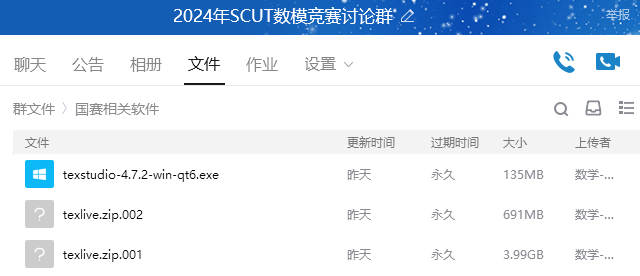
\includegraphics[width=.5\textwidth]{Download_Softwares.png} %图片的名称或者路径之中有空格会出问题 
     \caption{Download TeX Live and and TeXstudio from our QQ group} % 图片标题 
     \label{fig3}%交互引用
 \end{figure}
 
 \subsection{Installation and manual configuration}
 
 We first install TeX Live. In fact, one needs to unzip the ISO image (texliv.iso) and extract the contents of the ISO image to the computer system. Then you could execute the Windows batch file (install-tl-windows.bat) as an administrator. You can change the installation root if needed. It shall not, however, include any Chinese character, particularly the user's name. More than anything, remember the installation root needed for manual configuration.
 
 We are now ready to install TeXstudio. One just runs the executable file (texstudio-4.7.2-win-qt6.exe) as an administrator and keeps a shortcut on your desktop or quick launch toolbar.
 
 After the installation, we make the following configurations.
 
 \begin{itemize}
     \setlength{\parsep}{0ex} %段落间距
     \setlength{\topsep}{2ex} %列表到上下文的垂直距离
     \setlength{\itemsep}{1ex} %条目间距
     \item Open TeXstudio $\to$ Options $\to$ Configure TeXstudio
     \item General $\to$ Language
     \item Commands $\to$ Browse program $\to$ texlive $\to$ 2023 $\to$ bin $\to$ windows
     
     (LaTeX, PdfLaTeX, XeLaTeX, LuaLaTeX, BibTex, Biber)
     \item Click OK button
 \end{itemize}
 
 \subsection{Online \LaTeX ~writing tool: Overleaf}
 
 Overleaf is an online LaTeX writing tool that allows you to easily create and collaborate on perfectly formatted scientific and technical documents. You could get started by using a Google or ORCID account, or register it using your email. Then you can log in and use it online. Here is the link \href{https://www.overleaf.com/}{\underline{https://www.overleaf.com/}}.
 
 \begin{figure}[htbp]  %h此处,t页顶,b页底,p独立一页,浮动体出现的位置
 \centering
 \subfigure[Tex Studio]{
     \begin{minipage}[t]{0.4\linewidth}
         \centering
         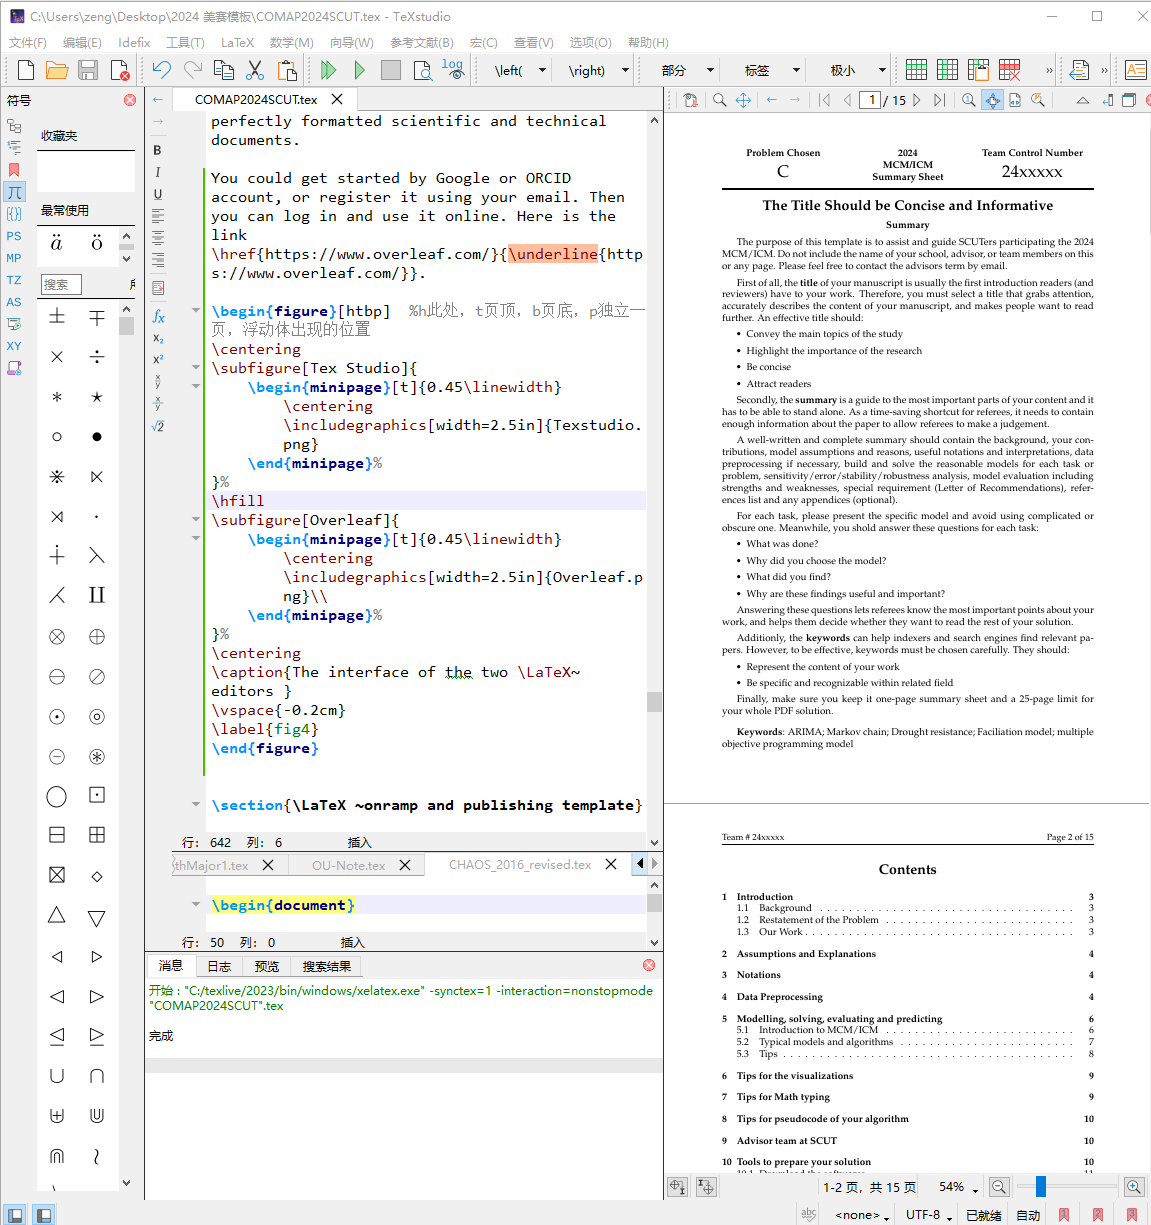
\includegraphics[width=2in]{Texstudio.png}
     \end{minipage}%
 }%
 %\hfill
 \subfigure[Overleaf]{
     \begin{minipage}[t]{0.4\linewidth}
         \centering
         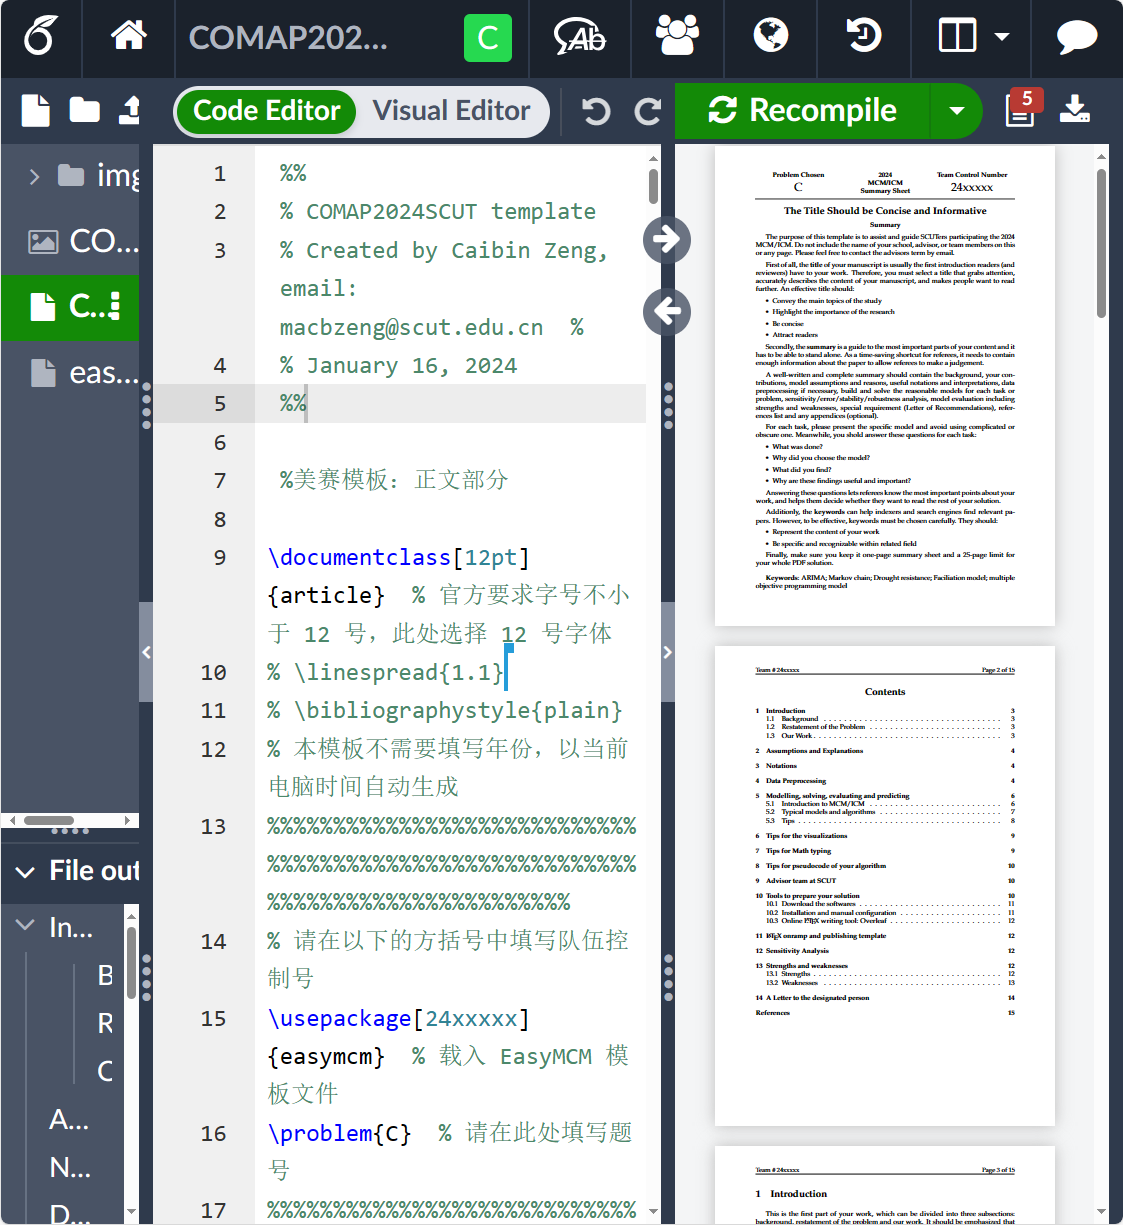
\includegraphics[width=2in]{Overleaf.png}\\
     \end{minipage}%
 }%
 \centering
 \caption{The interface of the two \LaTeX ~ editors }
 \vspace{-0.2cm}
 \label{fig4}
 \end{figure}
 
 
 \section{\LaTeX ~onramp and publishing template}
 
 You can check Zhihu or Bilibili for many documents
 and videos, so we are not going to elaborate any further. Nevertheless, the following useful documents are provided. 
 
 \begin{itemize}
     \setlength{\parsep}{0ex} %段落间距
     \setlength{\topsep}{2ex} %列表到上下文的垂直距离
     \setlength{\itemsep}{1ex} %条目间距
     \item \href{https://zhuanlan.zhihu.com/p/508559139}{\underline{https://zhuanlan.zhihu.com/p/508559139}}
     \item \href{https://yun.weicheng.men/Book/LaTeX%E5%85%A5%E9%97%A8.pdf}{\underline{https://yun.weicheng.men/Book/LaTeX入门.pdf}}	
     \item 
     \href{https://www.bilibili.com/video/BV1s7411U7Pr/?spm_id_from=333.337.search-card.all.click}{\underline{Bilibili video on a primer of \LaTeX}}
 \end{itemize}
 
 As mentioned in the summary part, this template aims to assist and guide SCUTers participating in the 2025 MCM/ICM. We will drift onto the source later and publish it. 
 
 
 
 \begin{mybox}{Caution}
     \begin{itemize}
         \setlength{\parsep}{0ex} %段落间距
         \setlength{\topsep}{2ex} %列表到上下文的垂直距离
         \setlength{\itemsep}{1ex} %条目间距
         \item If you use this template to complete your contest, please save your final submission as a PDF named 25XXXXX.pdf. (25XXXXX is your team control number, which is seven digits beginning with 25.)
         \item Please do no spread or publish this template out of our campus. 
         \item When you encounter problems using this template, contact your advisor or me directly by email.
     \end{itemize}
 \end{mybox}
 
  
 
 \begin{table}[htbp]
     \begin{center}		
         \caption{Advisor team at SCUT (2025)}
         \begin{tabular}{rlrl} % 居左对齐
             \toprule[2pt]
             \multicolumn{1}{m{2cm}}{\centering Name}
             &\multicolumn{1}{m{4cm}}{\centering Email}	& \multicolumn{1}{m{2cm}}{\centering Name}
             &\multicolumn{1}{m{4cm}}{\centering Email}\\ %3cm 和 8cm 是列宽,根据实际需求修改
             \midrule
             Shenquan Liu   & \href{mailto:mashqliu@scut.edu.cn}{mashqliu@scut.edu.cn} & Caibin Zeng & \href{mailto:macbzeng@scut.edu.cn}{macbzeng@scut.edu.cn}\\
             Weijian Ding   & \href{mailto:wjding@scut.edu.cn}{wjding@scut.edu.cn} & Xiaolan Liu & \href{mailto:liuxl@scut.edu.cn}{liuxl@scut.edu.cn} \\
             Xinhui Mao   & \href{mailto:maoxinhui@scut.edu.cn}{maoxinhui@scut.edu.cn} & Yongkuan Cheng & \href{mailto:chengyk@scut.edu.cn}{chengyk@scut.edu.cn} \\
             Bo Xie   & \href{mailto:xieb@scut.edu.cn}{xieb@scut.edu.cn} & Yuanpeng Zhu & \href{mailto:ypzhu@scut.edu.cn}{ypzhu@scut.edu.cn} \\
             Le Han   & \href{mailto:hanle@scut.edu.cn}{hanle@scut.edu.cn} & &\\
             \bottomrule[2pt]
         \end{tabular}	\label{tab4} % 交互引用
     \end{center}
 \end{table}
 
 \section{Sensitivity Analysis}
 
 After solving the problems, one needs to carry out the sensitivity/error/robustness analysis.
 
 \begin{itemize}
     \setlength{\parsep}{0ex} %段落间距
     \setlength{\topsep}{2ex} %列表到上下文的垂直距离
     \setlength{\itemsep}{1ex} %条目间距
     \item Sensitivity analysis provides users of mathematical and simulation models with tools to appreciate the dependency of the model output from model input and to investigate how important is each model input in determining its output.
     \item Any data collected will be corrupted by errors; it is important to quantify these errors as the magnitude of the errors will influence the interpretation of the data. Errors arise in all four stages of the experimental process: calibration, acquisition, data analysis, and data combination.
     \item Robustness analysis is a tool for analyzing problem situations with high uncertainty and sequential decision-making. It measures the flexibility of alternatives and the compatibility of decisions and plans.
 \end{itemize}
 
 \section{Strengths and weaknesses}
 
 \subsection{Strengths}
 
 \begin{itemize}
     \setlength{\parsep}{0ex} %段落间距
     \setlength{\topsep}{2ex} %列表到上下文的垂直距离
     \setlength{\itemsep}{1ex} %条目间距
     \item Models: novelty, interpretability,  universality.
     \item Algorithms: effectiveness, efficiency, improvement.	
     \item Never add any subjective evaluation.
 \end{itemize}
 
 \subsection{Weaknesses}
 
 \begin{itemize}
     \setlength{\parsep}{0ex} %段落间距
     \setlength{\topsep}{2ex} %列表到上下文的垂直距离
     \setlength{\itemsep}{1ex} %条目间距
     \item Missing other potentially useful features. 
     \item Certain degree of arbitrariness in modelling.	
     \item Much more brief than the strengths in length and number.
 \end{itemize}
 
 
 
 \clearpage
 %另起一页继续写。这时,你最好使用“\clearpage” 
 \section{A Letter to the designated person}
 
 The section is optional as required, which summarize your results or strategies in a one- to two-page. Here below is an example extracted from Team \# 2318982.
 
 \noindent Dear Puzzle Editor/ Sir or Madam, 
 
 \noindent Based on the file you provided, we have performed some interesting analyses of the data to answer the questions you have asked.
 
 \noindent First, we have developed a time series model ARIMA, which is the result of a rigorous selectionand iterative comparison of parameters. We are confident that this model will perform well infuture forecasts. According to this model, the number of reported results on March 1, 2023 will bebetween 10517 and 27007, with the number 16529 being particularly likely. This shows the strongvitality of wordle. In this era of bombardment of various games and short videos, it is surprisingthat a game still has such a high attention span one year after its launch. Moreover, with somevisualizations, we found that the number of wordle games gradually stabilized in Q3 2022 aftera crazy growth in Q1 2022. This means that a significant number of players have gotten used towordle games and made them part of their daily lives, rather than trying them once out of novelty.
 
 \noindent Next, we found that the percentage of hard mode is related to the attributes of the solution word.We conjecture that players will use the information shared by the community to decide whetherto turn on the Hard Mode. When players find that today’s wordle lacks challenge, Hard Mode ispreferred. After all, the rules of Hard Mode make the way to approach the correct answer moresingular.
 We also develop a Markov chain to model the process of players playing wordle games andpropose two game strategies. Finally, the prediction of the distribution of reported results at a futuredate is achieved by combining these results. Based on this model, the percentage distribution ofthe number of attempts for the word EERIE on March 1, 2023, showed a tendency to concentrateon three times and beyond, indicating the challenging nature of the word.
 \noindent Ultimately, we categorized the words according to their attributes. As we conjectured, theresulting word categories imply information about the difficulty of the words. Multi-syllabic,repeated-letter, objective, negative, and uncommon words are more difficult to guess than monosyllabic, emotionally rich, and common ones. From this we predict that the word EERIE will be agreat challenge for players, in line with the results of the Markov chain model we have developed.
 
 \noindent In the process of solving the problem, we found some interesting features of this dataset. Forexample, the increase or decrease in the number of reported words may be due to the difficulty orease of the word that day; words that are easy to guess correctly often contain common letters suchas a, t; results misrepresentation or answer leakage may occur.
 
 \noindent Many players say that Wordle has become the first warm-up for their brains when they wakeup. This is all due to your constant efforts to create a good gaming atmosphere and a harmoniousgaming community. Here, everyone is able to share their achievements freely and happily withoutbeing dramatized. We sincerely thank you for your efforts and hope that our analysis will help you.
 
 \hfill Sincerely,
 
 \hfill Team \# 2318982
 
 % 参考文献,务必统一格式,下面以书籍、期刊文章、网页资料为例
 \clearpage   %另起一页继续写。这时,你最好使用“\clearpage” 
 
 \begin{thebibliography}{99}
     
   %% 书籍
   \bibitem{NDZY2021}
   H. Ni, X. Dong, J. Dong, G. Yu, An Introduction to Machine Learning in Quantitative Finance, World Scientific, 2021.
   
   %% 期刊文献
   \bibitem{V2020}
   P. Virtanen et al., SciPy 1.0: fundamental algorithms for scientific computing in
   Python, Nature Methods, 17, 261--272, (2020).
   
   %% 网页资料
   \bibitem{Mesevage2021}
   T.G. Mesevage, What is data preprocessing \& What are the steps involved? (2021) \href{https://monkeylearn.com/blog/data-preprocessing/}{https://monkeylearn.com/blog/data-preprocessing/}
 \end{thebibliography}
 
 % \includepdf[pages={1,2}]{Memo.pdf} 
 
 \end{document}  % 结束